\noindent\textbf{Question 1:}

\noindent\emph{You (as a student who likes to travel) want to visit the 100 biggest cities in Germany. Since you have almost no time between two PCR assignments, you need to find the shortest possible routes between the cities in order to spend the least time for your travel. Luckily, the PCR course helps you to find a solution for this problem.
Your task in this assignment is to find a good solutions using the algorithms and techniques that you have covered in class. You can choose whatever algorithm your prefer, but the algorithm should provide a solution in a couple of minutes. Your start and goal city is Bonn.}

This week we were to solve the commonly known Travelling Salesman Problem. The TSP problem is of great interest to computer scientists because it belongs to the problem space known as NP. Non Deterministic Polynomial time. It generally means they're hard to solve, because every possibility must be taken into account. And the time it takes to solve a problem grows non polynomially with respect to the size of the problem. 

The problem is to find the guaranteed and provable optimal tour through all vertices in a fully connected graph, all possibilities must be explored and all combinations must be explored. The Travelling Salesman problem the cities can be thought of as vertices in a graph, and every city is connected to every other city via roads. The roads are edges in our graph, and as it is fully connected every vertex is connected to every other vertex. The travelling salesman problem need not have a fully connected graph, but the solution to the TSP should be general and thus the worst case is a fully connected graph.  

I solved the problem using C with only the stdio.h stdlib.h, time.h, math.h libraries. All structures and methods were ``homegrown'' using pointers, pointers to pointers and all that malloc goodness. Unfortunately it seg-faults periodically when I run the Simulated Annealing for over 10 iterations. The error was never found but sometimes it will run for nearly 100 iterations without seg faulting. Ah the fun that is pointers and memory management. The code consists of nearly 400 lines. At least half are due to comments, because working with pointers it's easy to get lost, and there are likely 100 lines of print statements commented out for debugging. There is a 60 line function to draw nice output in PostScript language. PS is a joyful stack orientated language. My program tsp.c when compiled and linked properly expects pairs of numbers from standard in, these are the x,y coordinates. The output can be piped to a new PostScript file to see the resulting path. The data provided was read with numpy and the vectors were normalized  to have data between 0 and 1, then the output is scaled to a 512 by 512 unit box. Germany is between 47 and 55 north, and 5 and 15 east, so the normalization to the x values is: $x = x-47/8  $ and for similar for y. So the x and y axis are not to the same scale. The numbers indicate the order the point was read from file, (to know which city) and the order in that version of the path.



% germany_100_greedy.pdf		
% my_samples_raw.pdf
% germany_100_swap.pdf		
% my_samples_simple_greedy.pdf
% my_samples_partial_sa.pdf


\begin{figure}[htbp]
  \centering
  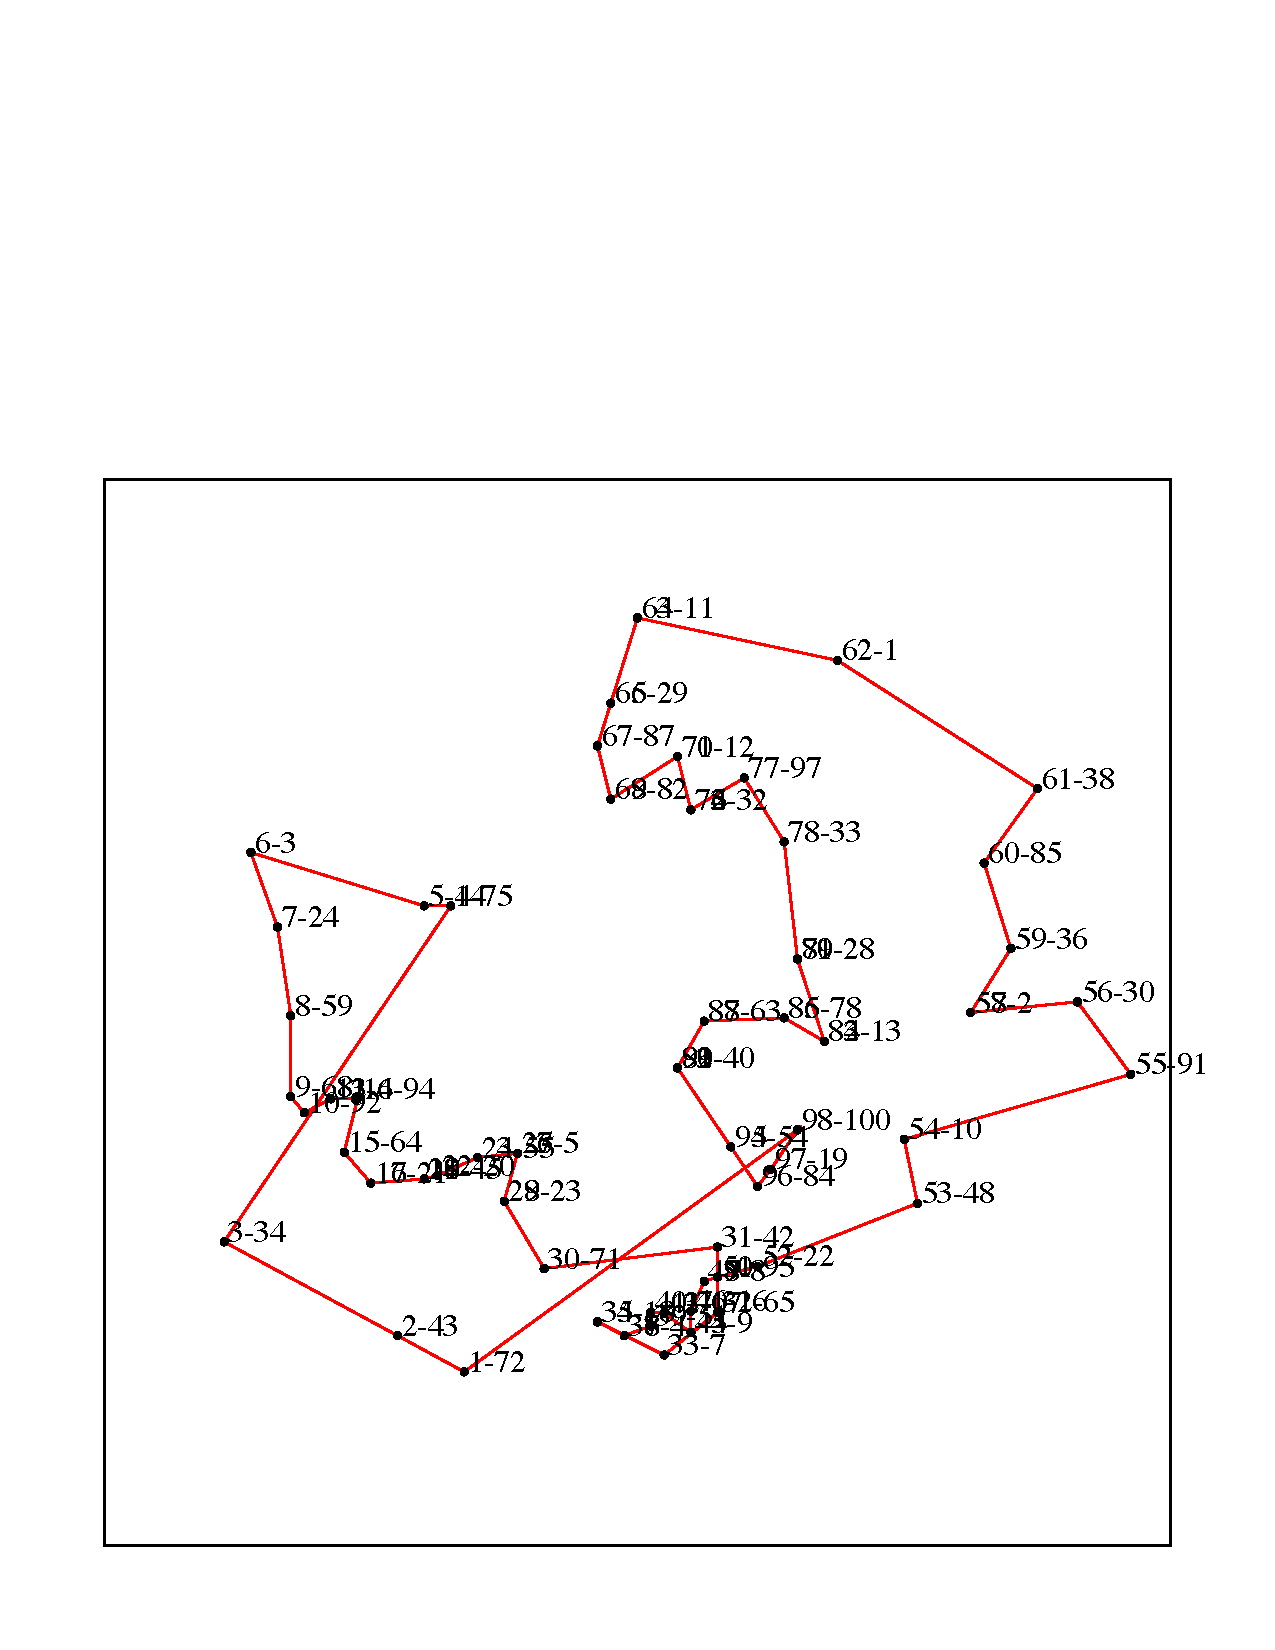
\includegraphics[width=1.0\textwidth]{./media/germany_100_greedy.pdf}
  \caption{ \label{Figure_1} Germany data tour found with Greedy nearest first algorithm.}
\end{figure}

\begin{figure}[htbp]
  \centering
  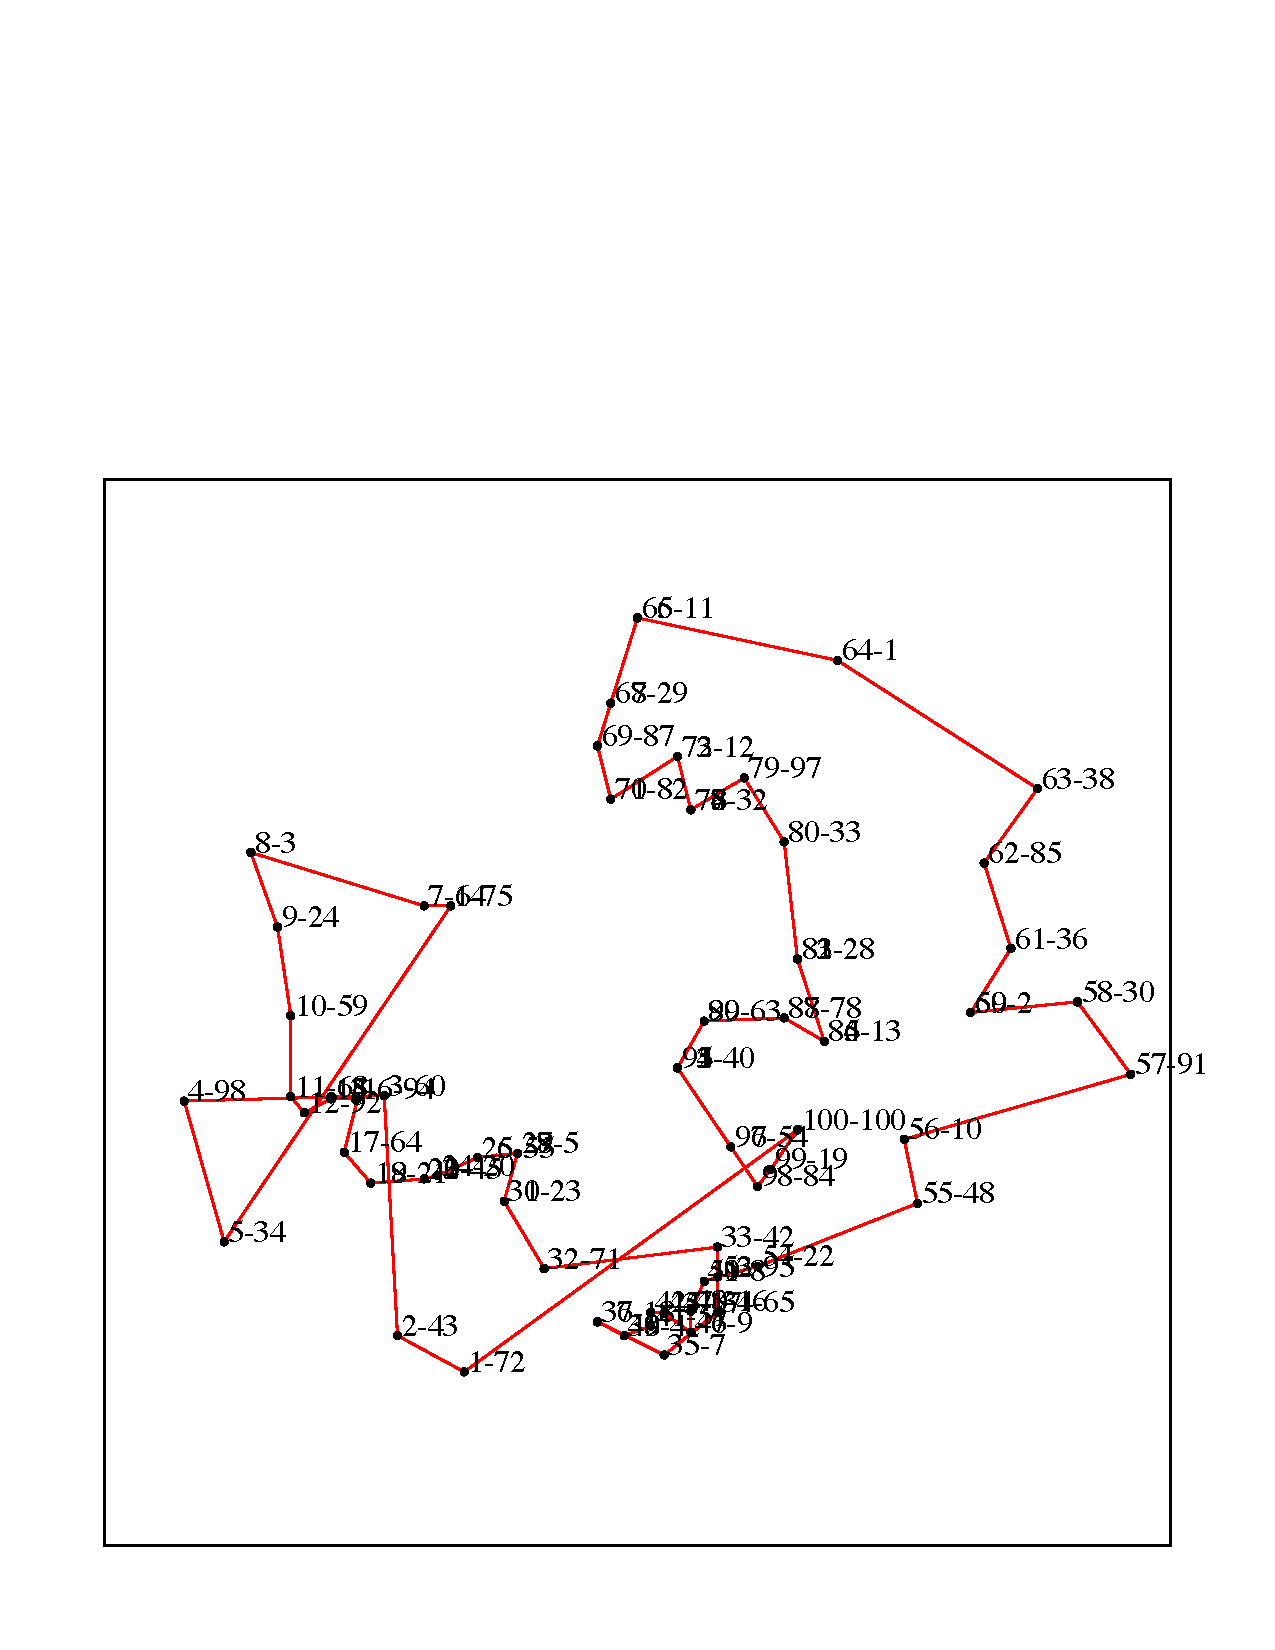
\includegraphics[width=1.0\textwidth]{./media/germany_100_swap.pdf}
  \caption{ \label{Figure_1} Germany data with a swap from Simulated Annealing, not completely finished but the program later seg faulted.}
\end{figure}

\begin{figure}[htbp]
  \centering
  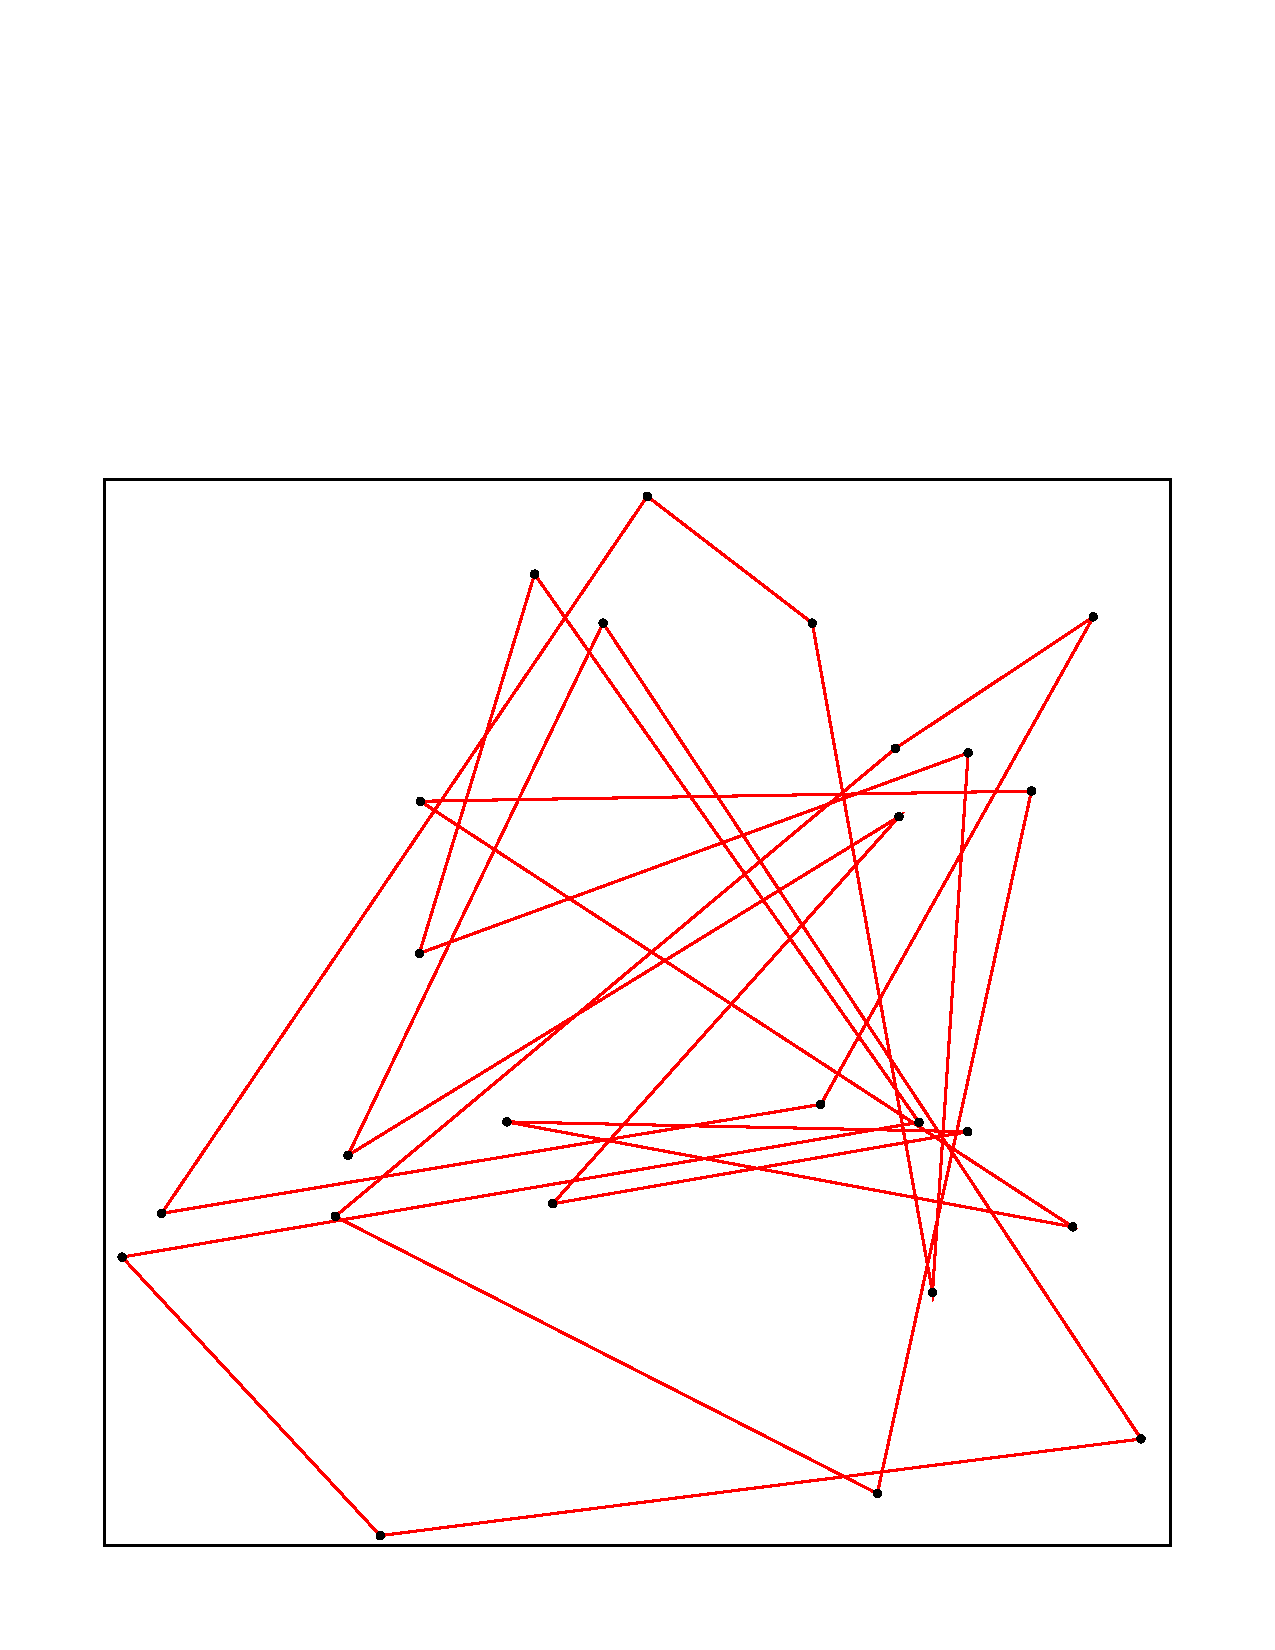
\includegraphics[width=1.0\textwidth]{./media/my_samples_raw.pdf}
  \caption{ \label{Figure_1}Some random data generated with python for testing initial state.}
\end{figure}

\begin{figure}[htbp]
  \centering
  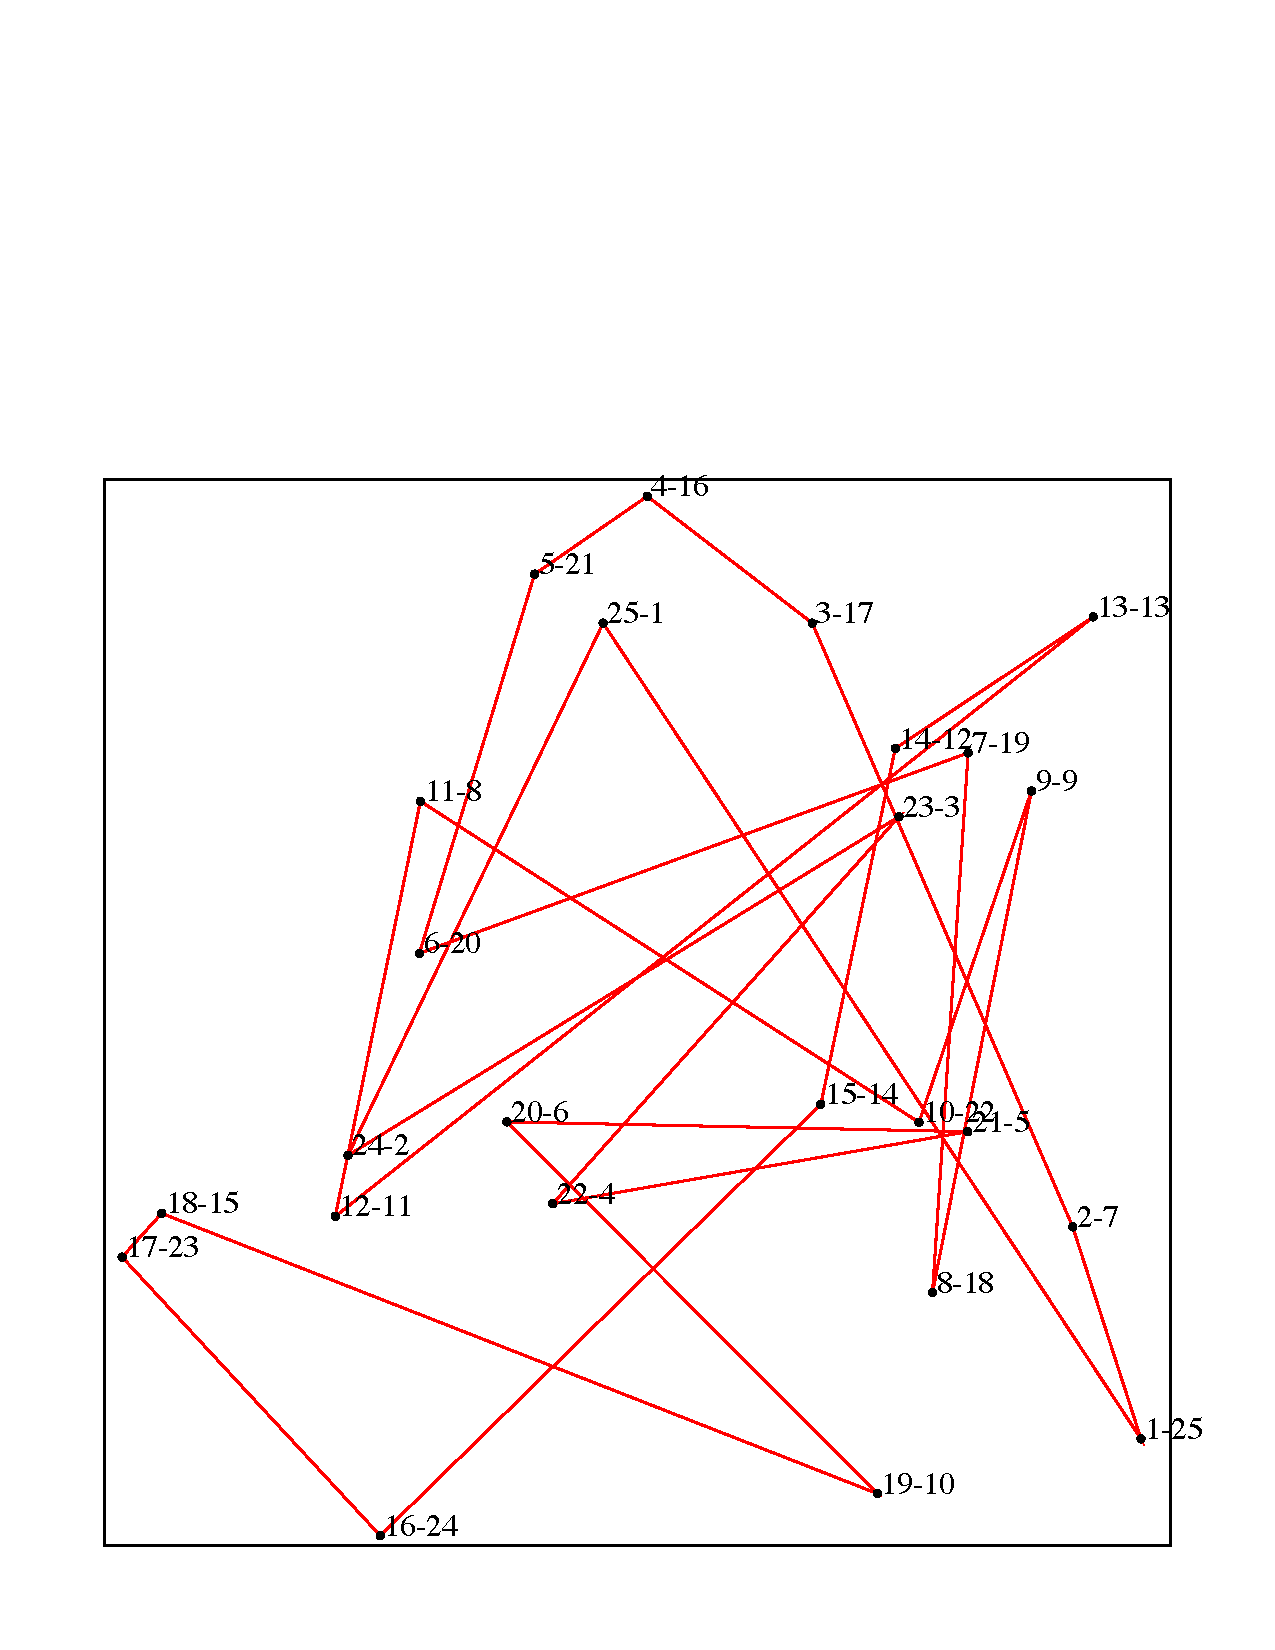
\includegraphics[width=1.0\textwidth]{./media/my_samples_partial_sa.pdf}
  \caption{ \label{Figure_1} Data above after 10 iterations of Simulated Annealing}
\end{figure}


\begin{figure}[htbp]
  \centering
  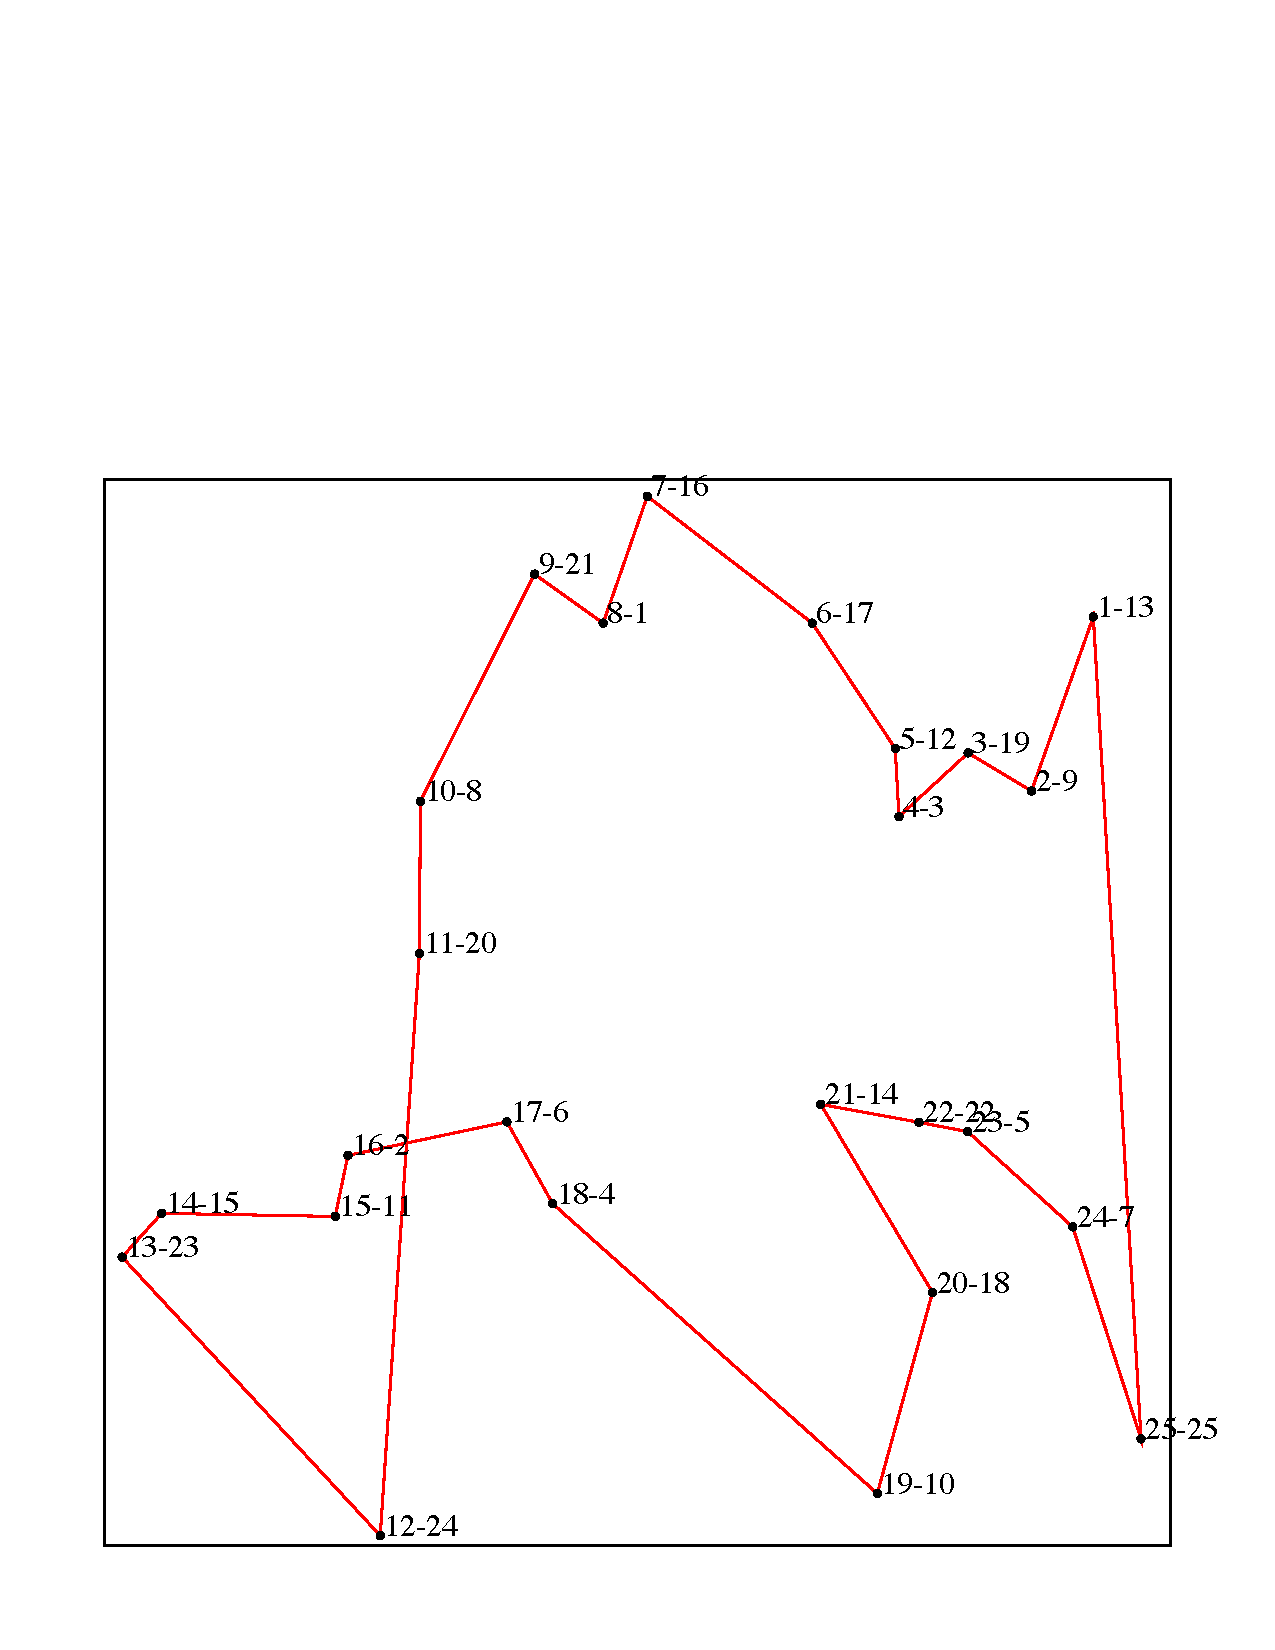
\includegraphics[width=1.0\textwidth]{./media/my_samples_simple_greedy.pdf}
  \caption{ \label{Figure_1}Same data as above with nearest first.}
\end{figure}


